\subsection{Análisis de WiFi}

\subsubsection{Velocidad}

Se tomaron medidas de velocidad a lo largo del día y se observó una disminución en ciertos periodos de alta ocupación.

\begin{figure}[H]
  \centering
  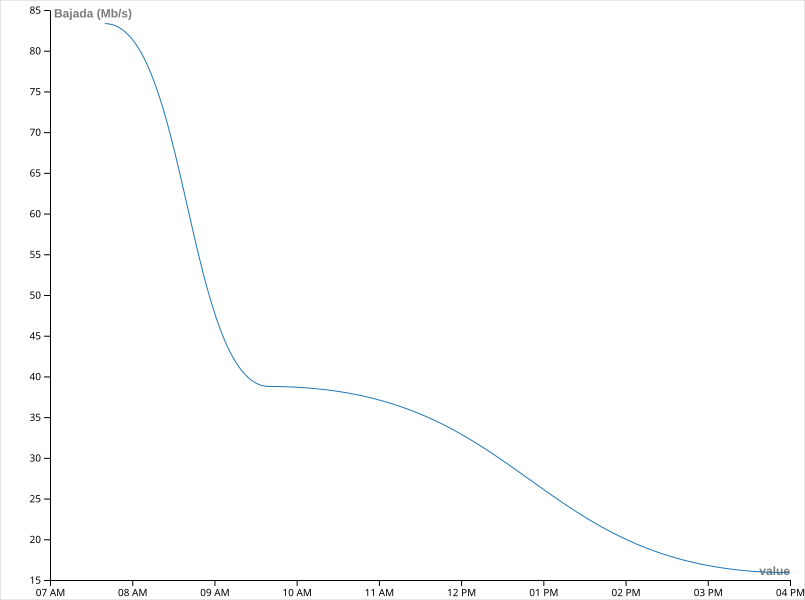
\includegraphics[width=0.7\textwidth]{../images/data-wifi-strength.png}
  \caption{Gráfica de análisis de la señal y velocidad de WiFi a lo largo del día.}
  \label{fig:wifi-strength}
\end{figure}

\subsubsection{Canales de red}

Analizando el ruido con utilidades de terminal se identificaron los siguientes canales y el número de dispositivos detectados:

\begin{table}[H]
  \centering
  \caption{Canales detectados y dispositivos}
  \label{tab:wifi-channels}
  \begin{tabularx}{0.6\textwidth}{c c}
    	\toprule
    Canal & Dispositivos detectados\\
    \midrule
    1 & 3\\
    2 & 1\\
    3 & 2\\
    4 & 1\\
    5 & 1\\
    6 & 5\\
    8 & 3\\
    9 & 2\\
    11 & 6\\
    36 & 1\\
    52 & 1\\
    64 & 1\\
    104 & 1\\
    149 & 4\\
    \bottomrule
  \end{tabularx}
\end{table}

\begin{figure}[H]
  \centering
  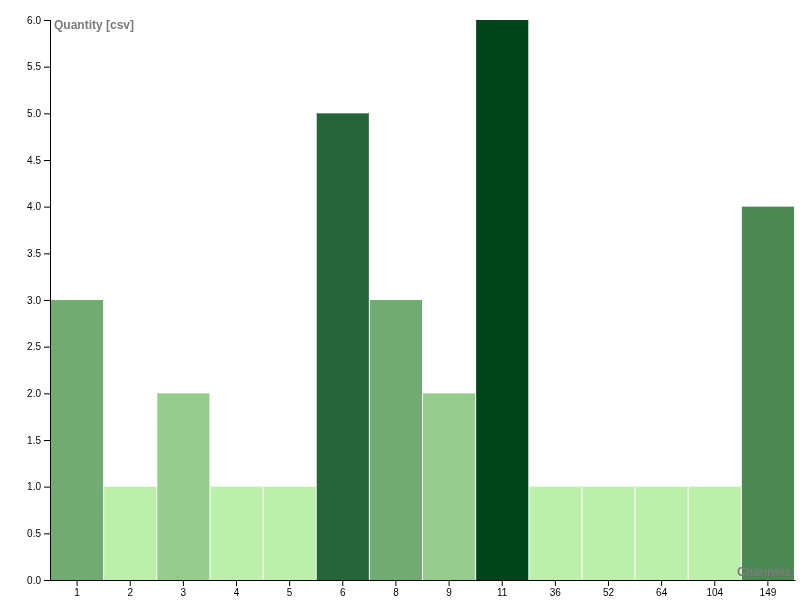
\includegraphics[width=0.6\textwidth]{../images/wifi-channels.png}
  \caption{Distribución de uso de canales detectados.}
  \label{fig:wifi-channels}
\end{figure}

Con estos resultados se recomienda priorizar el uso de canales en el rango 36--52 (banda de 5 GHz), ya que presentan menor interferencia y mayor capacidad para agregar dispositivos; la banda de 2.4 GHz (canales 1--11) muestra mayor saturación y debe emplearse solo cuando los equipos no soporten 5 GHz.
